\documentclass[11pt,a4paper]{article}
\ifdefined\PREPRINT\usepackage[preprint]{acl}\else\usepackage[review]{acl}\fi   % preprint.tex sets \PREPRINT
\usepackage{times}
\usepackage{latexsym}
\usepackage[T1]{fontenc}
\usepackage[utf8]{inputenc}
\usepackage{microtype}
% \usepackage{inconsolata}  % optional in the ACL template; enable on Overleaf
\usepackage{graphicx}
\usepackage{booktabs}
\usepackage{amsmath,amssymb}
\usepackage{xcolor}
\usepackage{subcaption}

\newcommand{\todo}[1]{\textcolor{red}{[TODO: #1]}}
\newcommand{\vviii}[1]{\textcolor{blue}{[v8: #1]}}
\newcommand{\PP}{PersonaPlex}
\newcommand{\hit}{hit@5}

\title{Do Full-Duplex Speech Models Listen in Text?\\
A Latent Transcript of the User and a Voice Gate That Closes It}

\ifdefined\PREPRINT
\author{Mikhail Kulik \\
  Independent Researcher \\
  \texttt{kulik.mr@phystech.edu}}
\else
\author{Anonymous submission}
\fi

\begin{document}
\maketitle

\begin{abstract}
Full-duplex speech models such as Moshi listen and speak at the same time, but emit text only for their \emph{own} speech.
Do they nevertheless represent what the \emph{user} says as text?
Applying logit and tuned lenses to Moshi and \PP, we find a latent transcript of the user in layers 21--30: the text head ranks the current user word among its top five for 46--48\% of content words above a matched control, on read and meeting speech alike, while the output stays silent.
The word becomes readable about 150\,ms before it ends, predictable words are favoured, and errors share form rather than meaning with the target; a tuned lens finds a word code from layer 12.
This transcript is closed by a \emph{voice gate}: while the model speaks, it loses 50--77\% of its readout of the user.
The gate is triggered by speech-like audio in the model's own channel, including time-reversed speech and the model's own generated replies, but hardly by noise, an echo of the user, or a second talker in the user's channel, and activation patching shows that it is set up in layers 1--8.
Ablating the transcript barely changes the reply, and the gate's behavioural effect is weaker and less specific than its effect on the representation: the transcript is readable but hardly used.
\end{abstract}

\section{Introduction}

Spoken dialogue models have moved from cascades of recognition, language model and synthesis to single networks that consume and produce audio tokens.
Full-duplex models go one step further: Moshi \citep{defossez2024moshi} and its fine-tuned descendant \PP{} \citep{roy2026personaplex} process the user's audio and their own audio as parallel streams at every 80\,ms frame, so that they can interrupt, back-channel and be interrupted.
To keep linguistic quality, Moshi predicts an aligned \emph{inner monologue}, a text stream that transcribes the model's own speech one frame ahead of its audio.
There is no comparable text stream for the user.
The model is never asked to transcribe its interlocutor.

This raises a basic question about how such systems understand speech: \emph{do they listen in text?}
Recent work found that interleaved speech--text language models latently map spoken words to their text tokens \citep{sternberg2026interleaved}, in the spirit of the observation that multilingual LLMs ``work in English'' in their middle layers \citep{wendler2024llamas}.
Full-duplex models pose the question in a sharper and more consequential form.
First, the text head is trained only on the model's \emph{own} words, so any reading of the \emph{user's} words through it is a zero-shot transfer across streams.
Second, the model often speaks while the user speaks, so one can ask what happens to its listening when it is talking, a situation that is central to turn-taking and barge-in \citep{lin2025fdb,lin2025fdb2} and that has a well-known analogue in human speaking-induced auditory suppression \citep{houde2002modulation}.

We answer these questions with lenses on the residual stream of the temporal transformer, using only teacher-forced forward passes that fit on two consumer GPUs.
Our contributions are:
\begin{itemize}
\setlength\itemsep{0pt}
\item \textbf{A latent transcript of the user} (\S\ref{sec:transcript}). In both models the text head reads the user's current word out of layers 21--30 while the output stays silent; the effect replicates on spontaneous meeting speech and vanishes on time-reversed speech.
\item \textbf{Its time course and content} (\S\ref{sec:what}). The word becomes readable before it ends, more so for predictable and frequent words, and its errors are cohort-like, favouring form over meaning. A tuned lens finds an earlier code, from layer 12, that generalises to target tokens it was never trained on.
\item \textbf{A voice gate} (\S\ref{sec:gate}). When the model speaks, the user's transcript is suppressed by up to three quarters. Controlled manipulations show that the gate is keyed to speech-like audio in the model's own channel, not to the content of what the model says, not to acoustic energy, not to an echo of the user, and not to a second voice in the user's channel; it persists for the model's own generated replies, and activation patching locates its onset in layers 1--8.
\item \textbf{Readable is not used} (\S\ref{sec:causal}). Removing the latent words from the residual stream changes the first word of the model's reply by 1--6\% of the effect of muting the user. While the model speaks, the user's audio shapes the reply less, but this behavioural reduction also occurs with a second talker in the user's channel.
\end{itemize}
\ifdefined\PREPRINT Code, notebooks and per-item results: \url{https://github.com/gglenpoi/listen-in-text}.\else All code and per-item results will be released.\fi

\section{Related work}

\paragraph{Full-duplex spoken dialogue.}
dGSLM \citep{nguyen2023dgslm} modelled two-channel dialogue with dual-tower transformers over discrete units.
Moshi \citep{defossez2024moshi} combined a text-pretrained 7B backbone, the Mimi codec and an inner-monologue text stream, and \PP{} \citep{roy2026personaplex} adds voice and role conditioning on top of it.
Data pipelines for speaker-separated dialogue \citep{nakata2026dialoguesidon,nakata2026duplexchat} and benchmarks for turn-taking and interruption \citep{lin2025fdb,lin2025fdb2} evaluate these systems behaviourally; we look inside them.

\paragraph{Text inside speech language models.}
Layer-wise analyses of self-supervised speech encoders find phonetic and then word-level information in intermediate layers \citep{pasad2021layerwise}.
For speech language models, scaling studies argue that text pretraining and speech--text interleaving drive semantic ability \citep{cuervo2024scaling,maimon2025scaling}, and \citet{sternberg2026interleaved} show with lens methods that interleaved models latently transcribe the speech they read.
We study a different architecture and setting, a full-duplex model whose text head is trained on its own speech only, and we add the interaction between listening and speaking, which does not arise in single-stream models.

\paragraph{Lenses, probes and causal tests.}
The logit lens decodes intermediate states with the model's own unembedding \citep{nostalgebraist2020logitlens}; the tuned lens learns a per-layer affine translator \citep{belrose2023tuned}.
Learned probes may report what they can decode rather than what the model uses \citep{hewitt2019control,belinkov2022probing}, which we address with shuffled-label lenses, held-out target tokens, and amnesic-style ablations that project directions out of the residual stream \citep{ravfogel2020null,elazar2021amnesic}.

\section{Method}
\label{sec:method}

\paragraph{Models.}
Moshi (\texttt{moshiko}) and \PP{}-7B share one architecture: a 32-layer temporal transformer (width 4096) runs over 17 token streams at 12.5\,Hz, namely the model's text stream, eight codebooks of the model's audio, and eight codebooks of the user's audio, all produced by the Mimi codec; a small depth transformer, which we do not use, predicts audio codebooks within a frame.
The text head is $\mathrm{logits}=W\,\mathrm{RMSNorm}(h_{32})$.
\PP{} is conditioned by a text prompt during which the user stream carries a sine tone; we use the prompt ``You enjoy having a good conversation.'' Moshi receives no prompt.

\paragraph{Inputs.}
We take 80 user turns of up to 20\,s from LibriSpeech test-clean \citep{panayotov2015librispeech} (read speech) and from the AMI meeting corpus, individual headset mix, test split \citep{carletta2005ami} (spontaneous speech).
Each turn is encoded with Mimi and placed on the user stream after a short silence, with the delays used in training.
In the default \emph{listen} condition the model's audio stream carries Mimi silence and its text stream padding, as when the model listens quietly; we checked that the model's own text head indeed outputs padding throughout the user's turn.
All forward passes are teacher-forced, so that every condition sees exactly the same user input.
Word boundaries come from forced alignment with MMS \citep{pratap2024mms}.

\paragraph{Readout.}
At layer $l$ we apply the final norm and the text head to the residual stream $h_l$ (logit lens), mask the four special tokens, and take the top five tokens.
A content word (at least four letters) counts as read out if the first SentencePiece token of the word appears in the top five at any frame between its onset and its offset plus a lag of four frames (320\,ms); as Mimi tokens are causal, frame $p$ has heard user audio up to frame $p{-}1$.
The \emph{control} scores the same word in a window of the same length in five random other turns, so that frequent tokens that the lens emits regardless of input do not count.
We report \hit{} \emph{excess}, readout minus control, with 95\% bootstrap intervals over turns.

\paragraph{Tuned lens.}
For layers $0,4,\dots,32$ we train a low-rank translator $T_l(h)=h+\bar h U_l V_l+b_l$ on RMS-normalised states $\bar h$ (rank 128), mapping every frame of a word to the first token of that word through the frozen final norm and head.
Training uses 70\% of the speakers of LibriSpeech test-clean, dev-clean and test-other (about 140 training turns); testing uses held-out speakers.
We report three tests of increasing strictness: \emph{unseen words}, \emph{unseen target}, in which the target token never occurred as a training target, and the same on AMI.
A lens trained on shuffled word labels serves as the control.

\paragraph{Own-channel manipulations.}
To create overlap, the model's own audio stream is filled with another turn of the same corpus (\emph{speech}) while its text stream keeps padding, so that only the sound differs from \emph{listen}.
Further conditions vary one property at a time: the same speech \emph{reversed} in time (no words, speech-like spectro-temporal structure), \emph{speech-shaped noise} with the same long-term spectrum and level (random phase), an \emph{echo} of the user's own turn delayed by 200\,ms at $-10$\,dB, the speech at attenuated levels ($-40$ to $-10$\,dB), and, in a separate run, own audio only or own text only.
We measure the paired drop of the user readout relative to \emph{listen}, and report it as the \emph{share of readout lost}.
As a two-talker control, the other speaker's speech is instead mixed into the \emph{user's} channel at 0 or $-10$\,dB relative to the user, with the own channel silent.

\paragraph{Natural overlap.}
To test the gate on the model's own speech, the model first hears a 6\,s user utterance and then freely generates its reply (text and all eight audio codebooks, sampled with Moshi's default temperatures) for 10.5\,s while the user is silent; replies with fewer than three text tokens are re-sampled up to three times.
A 10\,s user turn is then placed on the user stream 0.5\,s after the reply window opens, and the reply is teacher-forced in the own channel with its text (\emph{own reply}), with its audio only, or replaced by another speaker's speech; the baseline keeps the own channel silent in the same context.
Usable replies were obtained for 85--90\% of turns for \PP{} and 60--70\% for Moshi (12--18 turns, 170--243 words per corpus).

\paragraph{Activation patching.}
To locate the gate, we record, in the \emph{listen} run, the update that each layer's attention and MLP block adds to the residual stream at the frames of the user's turn, and substitute it, for a block of layers, into the run with speech in the own channel.
We report the share of readout restored at the readout layer, $(\hit_{\text{patch}}-\hit_{\text{speak}})/(\hit_{\text{listen}}-\hit_{\text{speak}})$, for whole layers, attention only, or MLP only (12 turns per corpus).

\paragraph{Causal tests.}
We force an end-of-padding token into the model's text stream 0.5\,s after the user's turn, which makes the model start speaking on the next frame, and read the distribution of its first word.
At each layer of a range we project out, at all frames of the user's turn, the subspace spanned by the directions of the user's words: rows of $W$ for a \emph{late} ablation (layers 22--30) or their pull-back through the tuned lens, $w+U(Vw)$, for an \emph{early} ablation (layers 12--30).
The control ablates the same number of words of other turns.
We report KL divergence of the first-word distribution and the change of the total probability of the heard words, $\Delta\log P(\text{heard})$; muting the user's stream is the positive control.

\section{Results}

\subsection{A latent transcript of the user}
\label{sec:transcript}

\begin{figure*}[t]
\centering
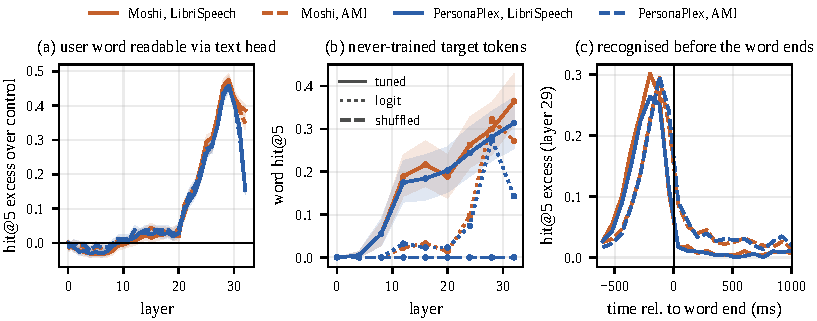
\includegraphics[width=\textwidth]{figures/fig1_readout.pdf}
\caption{\textbf{Where and when the user's words become text.} (a) Logit-lens readout of the user's current word, as \hit{} excess over a control, across layers; shading: 95\% bootstrap CI. (b) Tuned (solid), logit (dotted) and shuffled-label (dashed) lenses on target tokens never seen in tuned-lens training (LibriSpeech, held-out speakers). (c) Readout at layer 29 as a function of how much of the word has been heard, aligned to word offset.}
\label{fig:readout}
\end{figure*}

Figure~\ref{fig:readout}a shows the main result.
In the first twenty layers the text head reads nothing of the user.
From layer 21 the user's current word becomes readable, and at layers 28--30 the head ranks it among its top five tokens in excess of the control for 46\% (\PP) to 48\% (Moshi) of content words on LibriSpeech (\PP: 0.458 [0.441, 0.477]; Moshi: 0.476 [0.458, 0.493]) and to the same degree on AMI meetings (0.462 and 0.468).
The two models, which share pre-training but differ in fine-tuning, are almost indistinguishable.
The readout declines in the last layers, where the representation turns to the model's own next text token, which is padding.
On time-reversed user speech the excess is 0.03--0.05, so the readout depends on intelligible words rather than on any regularity of the input.

\subsection{When and what is recognised}
\label{sec:what}

\paragraph{Before the word ends.}
Aligned to word offset (Fig.~\ref{fig:readout}c), the readout peaks 120--200\,ms before the end of the word, that is about 120\,ms after its onset for a median content word of 340\,ms, and it disappears within 100\,ms after the word.
Readout before the word begins is close to zero ($+0.02$ at $-200$\,ms), which rules out pure prediction from context.
The latent transcript is therefore incremental and short-lived: it tracks the word currently heard rather than accumulating a record of the turn.

\begin{table}[t]
\centering\small
\setlength\tabcolsep{4pt}
\resizebox{\columnwidth}{!}{\begin{tabular}{lrrrr}
\toprule
Predictor & Moshi LS & Moshi AMI & PPlex LS & PPlex AMI \\
\midrule
surprisal (GPT-2) & -0.35$^{*}$ & -0.47$^{*}$ & -0.23$^{*}$ & -0.45$^{*}$ \\
frequency (Zipf) & +0.67$^{*}$ & +0.26$^{*}$ & +0.81$^{*}$ & +0.34$^{*}$ \\
duration & +0.24$^{*}$ & +0.12 & +0.36$^{*}$ & +0.01 \\
length & -0.24$^{*}$ & +0.21$^{*}$ & -0.37$^{*}$ & +0.25$^{*}$ \\
position in turn & +0.14$^{*}$ & +0.42$^{*}$ & +0.09 & +0.24$^{*}$ \\
\midrule
$n$ words & 1403 & 1298 & 1403 & 1298 \\
\bottomrule
\end{tabular}}
\caption{Which words are read out: standardised coefficients of a logistic regression of readout at the best layer. $^{*}$: 95\% bootstrap CI excludes zero.}
\label{tab:factors}
\end{table}

\paragraph{Predictable and frequent words.}
Table~\ref{tab:factors} shows that readout depends on the word.
Words that GPT-2 \citep{radford2019gpt2} finds surprising given the preceding words are read out less often, in all four settings, and frequent words \citep{speer2022wordfreq} more often; by surprisal tertile the readout falls from 0.68--0.74 to 0.36--0.41.
The listener thus combines bottom-up evidence with a strong prior from its language model, as human listeners do.

\begin{table}[t]
\centering\small
\setlength\tabcolsep{3pt}
\resizebox{\columnwidth}{!}{\begin{tabular}{lrrrr}
\toprule
Candidate & Moshi LS & Moshi AMI & PPlex LS & PPlex AMI \\
\midrule
same lemma & +0.215$^{*}$ & +0.187$^{*}$ & +0.174$^{*}$ & +0.165$^{*}$ \\
similar sound & +0.194$^{*}$ & +0.117$^{*}$ & +0.186$^{*}$ & +0.117$^{*}$ \\
similar meaning & +0.060$^{*}$ & +0.069$^{*}$ & +0.046$^{*}$ & +0.052$^{*}$ \\
sound + meaning & +0.021$^{*}$ & +0.025$^{*}$ & +0.018$^{*}$ & +0.029$^{*}$ \\
homophone & +0.003 & +0.001 & +0.003 & +0.001 \\
\midrule
meaning (sound-unlike) & +0.040$^{*}$ & +0.027$^{*}$ & +0.030$^{*}$ & +0.025$^{*}$ \\
sound (meaning-unlike) & +0.048$^{*}$ & +0.028$^{*}$ & +0.052$^{*}$ & +0.020$^{*}$ \\
\bottomrule
\end{tabular}}
\caption{When the target word is not in the top five: excess rate at layer 28 of top-five candidates related to the heard word, over the same relation to other words of the same turn. Relations from WordNet lemmas \citep{miller1995wordnet}, CMUdict phone edit distance and sentence-embedding similarity; the last two rows exclude the other relation. On reversed speech all rates are within $\pm0.015$. $^{*}$: CI excludes zero.}
\label{tab:nearmiss}
\end{table}

\paragraph{Cohort-like errors.}
When the target is not in the top five, the candidates that are there are related to it (Table~\ref{tab:nearmiss}).
Words with the same lemma are most frequent (+0.17 to +0.22 over a same-turn control), followed by similar-sounding words (+0.12 to +0.19); words of similar meaning are much rarer (+0.05 to +0.07), and meaning without sound similarity rarer still.
None of these relations is present for reversed speech.
Typical AMI examples are \emph{gonna}$\to$\emph{going}, \emph{yeah}$\to$\emph{yes}, \emph{write}$\to$\emph{right}, and \emph{things}$\to$\emph{stuff}.
Lemma relations are significant from layer 12, sound relations only from layer 24.
This pattern resembles the activation of a cohort of form-similar competitors in human spoken word recognition \citep{marslenwilson1987} more than a semantic paraphrase.

\paragraph{An earlier code.}
The logit lens sees nothing before layer 21, but a tuned lens does (Fig.~\ref{fig:readout}b).
On target tokens it was never trained to output, the tuned lens at layer 12 reads 18--19\% of words (\PP{} 0.175 [0.129, 0.226], Moshi 0.189 [0.143, 0.240]) against 2--3\% for the logit lens and exactly zero for the shuffled-label lens; on AMI it reads 10--11\% (logit lens 3--4\%).
For held-out speakers and unseen words with seen targets it reaches 0.37 at layer 12.
Lexical identity is therefore linearly present at least nine layers before it aligns with the text head, and the translator that exposes it generalises across tokens and corpora.

\subsection{A voice gate}
\label{sec:gate}

\begin{figure*}[t]
\centering
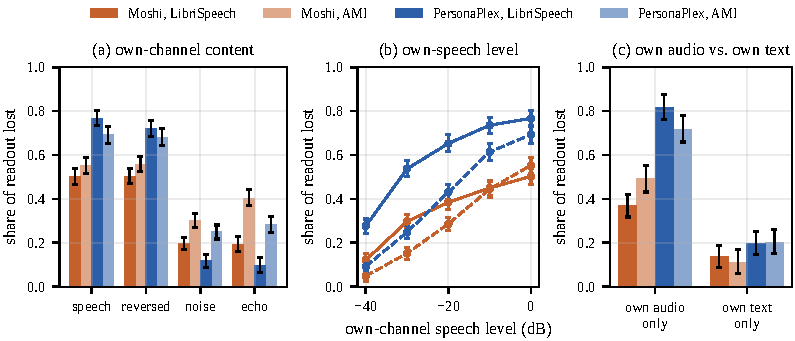
\includegraphics[width=\textwidth]{figures/fig2_gate.pdf}
\caption{\textbf{The voice gate.} Share of the listen-condition readout of the user lost when the model's own channel carries (a) another speaker's speech, the same speech reversed, speech-shaped noise, or a 200\,ms echo of the user; (b) speech at different levels (0\,dB is the natural level); (c) only the audio or only the text of the model's own speech. Error bars: 95\% bootstrap CI; layer of peak readout.}
\label{fig:gate}
\end{figure*}

Full-duplex models speak while they listen.
When the model's own channel carries speech during the user's turn, its readout of the user drops by 77\% (\PP, LibriSpeech; 69\% on AMI) and by 50--55\% (Moshi) (Fig.~\ref{fig:gate}a).
Because the user input is identical across conditions, this is a paired effect on the same words.
It is not an artefact of the model's own words outcompeting the user's in the top five: excluding the tokens of the model's own speech from the ranking leaves the loss at 67--73\% (\PP) and 40--44\% (Moshi).
The suppressed words have not moved elsewhere either: at the same layers the head now reads the model's \emph{own} speech (\hit{} excess 0.38 for \PP{}, 0.23--0.24 for Moshi), i.e., the latent transcript switches from the user to the model itself.

\paragraph{What closes the gate.}
Four manipulations of the own channel isolate the trigger.
(i) \emph{Audio, not text.} Own audio alone reproduces most of the loss (\PP{} 72--82\%, Moshi 37--49\%); own text alone causes only 10--20\% (Fig.~\ref{fig:gate}c).
(ii) \emph{Not what is said.} Time-reversed speech, which contains no words, suppresses as much as speech (\PP{} 72\%, Moshi 50--56\%).
(iii) \emph{Not energy.} Speech-shaped noise with the same spectrum and level suppresses far less (12--30\%).
(iv) \emph{Not the user's voice in the own channel.} A 200\,ms echo of the user at $-10$\,dB suppresses 10--40\%, whereas the other speaker's speech at the same level suppresses 45--74\%.
The loss grows monotonically with the level of the own speech (Fig.~\ref{fig:gate}b): already at $-40$\,dB \PP{} loses 28\% on LibriSpeech, at $-10$\,dB 74\%.
\PP{} gates more strongly than Moshi at every level on LibriSpeech.
The gate is transient: when the model's speech ends in the middle of a user turn, the readout recovers within about a second (Appendix~\ref{app:recovery}).

\begin{figure*}[t]
\centering
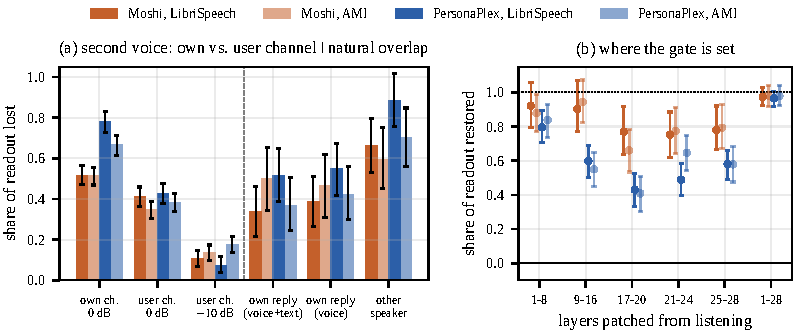
\includegraphics[width=\textwidth]{figures/fig5_v9.pdf}
\caption{\textbf{Specificity, natural overlap and locus of the gate} (layer 29). (a) Readout lost with another speaker in the model's own channel versus mixed into the user's channel (left), and, in a separate context, while the model hears its own freely generated reply (with its text or audio only) or another speaker (right). (b) Share of the readout restored when the listen-condition updates of a block of layers are patched into the run with own-channel speech. Error bars: 95\% bootstrap CI.}
\label{fig:v9}
\end{figure*}

\paragraph{Own channel, not a second talker.}
A second voice is not suppressive in itself: mixed into the user's channel at $-10$\,dB it costs only 8--18\% of the readout, whereas own-channel speech at the same level costs 45--74\% (Fig.~\ref{fig:v9}a); at equal level (0\,dB), where masking is substantial, the mix costs 35--43\% against 51--78\% in the own channel.
The suppression thus depends on \emph{which} channel carries the speech.

\paragraph{The model's own reply.}
The gate also closes when the model hears its own freely generated reply in its own voice and with its own inner monologue: the readout of the overlapping user turn drops by 52\% [39, 65] and 37\% [24, 51] for \PP{} and by 34\% [21, 46] and 50\% [35, 66] for Moshi (LibriSpeech, AMI), and by the same amount when the model's own words are excluded from the ranking.
Another speaker's continuous speech in the same context suppresses more (60--88\%), plausibly because generated replies contain pauses and do not cover the whole user turn.

\paragraph{Where the gate is set.}
Patching all layer updates of layers 1--28 restores the readout completely (97--98\%), so the raw embedding of the own channel plays no role by itself (Fig.~\ref{fig:v9}b).
Patching only layers 1--8 already restores 80--84\% for \PP{} and 88--92\% for Moshi, although nothing of the user is readable through the text head before layer 21; single later blocks restore less for \PP{} (41--65\%).
The gate is therefore set up early and inherited by the layers that form the transcript.
Neither component alone suffices: across layers 1--28, attention updates restore 36--63\% and MLP updates alone none; the same pattern holds for the model's own reply.

\subsection{Readable is not used}
\label{sec:causal}

\begin{figure}[t]
\centering
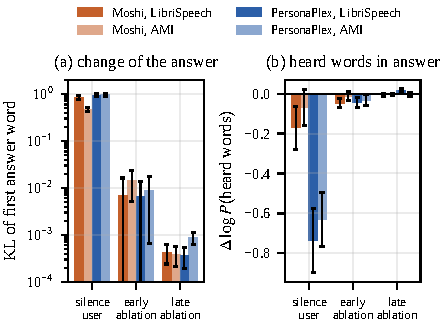
\includegraphics[width=\columnwidth]{figures/fig3_causal.pdf}
\caption{\textbf{Causal tests} on the first word of the model's reply. Muting the user changes it strongly; projecting the user's word directions out of layers 12--30 (early) or 22--30 (late) barely does, relative to ablating other turns' words. Log scale in (a).}
\label{fig:causal}
\end{figure}

Is the latent transcript the route by which the user's words reach the response?
Muting the user's stream changes the first word of the reply substantially (KL 0.94--0.95 for \PP, 0.46--0.85 for Moshi) and, for \PP, lowers the probability of the heard words by 0.63--0.74 nats (Fig.~\ref{fig:causal}).
Ablating the latent words has a far smaller effect.
The late ablation removes the logit-lens readout completely (\hit{} 0.53$\to$0.00) yet leaves the response unchanged (KL $\le 0.001$).
The early ablation removes the tuned-lens readout (0.95$\to$0.00) and most of the logit-lens readout (0.53$\to$0.19) and lowers $\log P(\text{heard})$ significantly but slightly, by 0.03--0.05 nats relative to the control ablation (\PP{} LibriSpeech $-0.043$ [$-0.067$, $-0.019$]; AMI $-0.031$ [$-0.060$, $-0.001$]; Moshi LibriSpeech $-0.046$; Moshi AMI n.s.), with KL 0.007--0.014.
That is 1--6\% of the effect of muting the user.
The user's words are thus available in text-aligned form, but the response draws on them mainly through other, non-lexical directions.

\paragraph{Does the gate change what the model says?}
If the transcript is hardly used, its suppression need not matter for behaviour.
We therefore repeated the forced-reply test with the user present or muted inside each own-channel condition, and measured the user's influence on the reply as $\mathrm{KL}(\text{user present}\,\|\,\text{user muted})$ for the first word, relative to the same quantity when the model listens (Fig.~\ref{fig:gatebeh}; 60 turns per corpus).
Comparing within a condition removes the effect of the model's own speech on the reply itself.
For \PP{} the user's influence falls to 46\% [40, 55] of its listening value on LibriSpeech and to 29\% [25, 34] on AMI when the model speaks, and to 48\% and 39\% for reversed speech, whereas speech-shaped noise leaves it at 103\% and 84\%.
Equivalently, muting the user changes the top first word in 98--100\% of turns while \PP{} listens but in only 47--65\% while it speaks.
For Moshi the influence falls to 52\% [46, 59] on LibriSpeech, but not significantly on AMI (93\% [78, 112]), where the user's influence on Moshi's reply is weak to begin with (KL 0.46), and reversed speech reduces it only slightly (88\% on LibriSpeech).
A repetition with 48 turns reproduced these values (\PP{} 43\% and 28\%, Moshi 51\% and 82\%), but also showed that this measure is not specific to the gate: with a second voice mixed into the user's channel, which barely affects the readout at $-10$\,dB, the user's influence also falls to 40--53\% for \PP{} (Moshi 49\% on LibriSpeech).
KL to a muted user mixes lexical content with the mere presence of a speaker, which matters for turn-taking.
The content-word measure is more selective but only reliable for \PP{} on LibriSpeech, where hearing the user raises the probability of its content words in the reply while the model listens ($+0.33$ nats) but not while it speaks ($-0.44$; difference $-0.76$ [$-0.99$, $-0.53$]); a $-10$\,dB second voice in the user channel reduces it less ($-0.28$ [$-0.47$, $-0.09$]).
For the model's own natural reply, the user's influence on \PP{}'s next turn is reduced moderately (KL retention 65\% [45, 88] and 72\% [39, 109]) and not at all for Moshi.
We conclude that the voice gate is a robust property of the representation, whose behavioural consequences are present but weaker and less specific than the representational effect.
Quieter own speech ($-30$\,dB) already reduces the influence on LibriSpeech (\PP{} 45\%, Moshi 70\%), but not for \PP{} on AMI.
Results for the echo condition are not interpretable in this design and are reported in Appendix~\ref{app:v8}.

\begin{figure}[t]
\centering
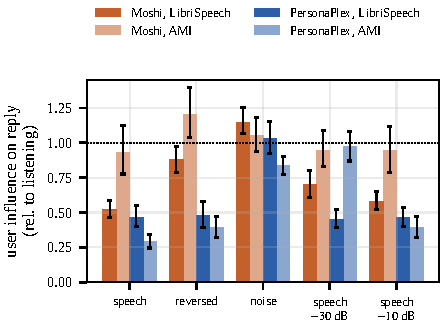
\includegraphics[width=\columnwidth]{figures/fig4_gate_behaviour.pdf}
\caption{\textbf{The gate in behaviour.} Influence of the user's audio on the first word of the reply, $\mathrm{KL}(\text{user present}\,\|\,\text{user muted})$, under each own-channel condition relative to listening (dotted line). Error bars: 95\% bootstrap CI of the ratio over turns.}
\label{fig:gatebeh}
\end{figure}

\section{Discussion}

\paragraph{Listening in text, partially.}
Both models carry a word-by-word, text-aligned transcript of their interlocutor that no objective asked for: the text head was trained only on the model's own speech, yet it transfers across streams.
This extends the finding that interleaved speech LMs latently transcribe their input \citep{sternberg2026interleaved} to full-duplex models and to spontaneous speech.
The transcript is fleeting, prior-driven and form-based, and is preceded by an earlier code that the tuned lens can translate.
Our ablations suggest, however, that it is a by-product of a shared text-aligned space rather than the channel through which the model understands; this is consistent with the general caution that decodable is not necessarily used \citep{hewitt2019control,elazar2021amnesic}.

\paragraph{The voice gate and turn-taking.}
The gate behaves like a learned speaking-induced suppression \citep{houde2002modulation}: in the representation it is triggered by speech-like sound in the model's own channel, regardless of content, and spares noise and an echo of the user; it does not arise from a second talker in the user's channel, and it is set up in early layers, which suggests a dedicated routing decision rather than late competition between transcripts.
For dialogue systems it has a direct implication.
A model that transcribes itself instead of the user while both speak is poorly placed to react to what is said during overlap, for example a correction or a stop request, which is exactly where current full-duplex benchmarks find weaknesses \citep{lin2025fdb,lin2025fdb2}.
The stronger gate of \PP{} suggests that fine-tuning can change the strength of this trade-off.
Readout under overlap is cheap to measure and could serve as a diagnostic during training, for instance when training on speaker-separated dialogue \citep{nakata2026dialoguesidon,nakata2026duplexchat}.

\section{Conclusion}
Full-duplex speech models listen partly in text: their user's words surface, briefly and before they end, in the text space of the backbone, are read cohort-style, and are switched off when the model hears itself speak.
The transcript is readable but hardly used, which separates a latent transcript from understanding.
The gate is specific to the model's own channel, holds for its own generated speech and is set up in early layers; its effect on behaviour is real but weaker and less specific, which makes the readout of the user under overlap a cheap and sensitive diagnostic of how well a full-duplex model listens while it talks.

\section*{Limitations}
We study two models of a single family that share pre-training, so we cannot tell whether the transcript and the gate are properties of full-duplex models in general or of Moshi's design with an inner monologue.
All inputs are English.
Most overlap conditions place another speaker's turn in the model's own channel under teacher forcing; our natural condition uses the model's own replies, but they were generated while the user was silent and then teacher-forced, so the model never reacts to the overlapping user, and the generated replies do not cover the user's turn completely.
Readout is scored on the first SentencePiece token of words of at least four letters, with a top-five criterion and a fixed lag; our controls guard against frequency effects but other choices would change absolute numbers.
The tuned lens is trained on about 140 turns, and better lenses could find the code even earlier.
Our causal tests remove only the directions of the heard words and read only the first word of a forced reply; information could be carried redundantly in directions we do not ablate, and longer responses might reveal larger effects.
The near-miss analysis relies on automatic resources (CMUdict, WordNet, sentence embeddings) with thresholds that we vary in the appendix but cannot validate against human judgements.

\section*{Ethics Statement}
We analyse publicly released models on public, licensed corpora (LibriSpeech, CC BY 4.0; AMI, CC BY 4.0) and collect no new data from people.
Our findings concern how models represent speech and do not enable new capabilities; a better understanding of when full-duplex systems fail to attend to their users may help make them safer to interrupt.
All experiments ran on free cloud notebooks with two 16\,GB GPUs (NVIDIA T4); all experiments together used about 13.3 hours of GPU quota.

\bibliography{refs}

\appendix

\section{Readout after the model stops speaking}
\label{app:recovery}

\begin{figure}[h]
\centering
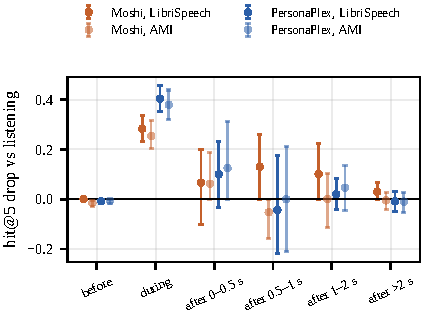
\includegraphics[width=\columnwidth]{figures/figA_recovery.pdf}
\caption{Readout drop relative to listening for user words heard before, during and after a stretch of the model's own speech that ends in the middle of the user's turn.}
\label{fig:recovery}
\end{figure}

When the model's own speech covers only part of the user's turn (Fig.~\ref{fig:recovery}), the readout of words heard before it is unaffected, the words heard during it lose 0.3--0.4 \hit{}, and words heard after it largely recover within one to two seconds, with wide intervals because few words fall in each bin.

\section{Implementation details}
\label{app:impl}
Weights are loaded tensor by tensor and split across two GPUs (16 layers each) in float16 on T4 and bfloat16 otherwise; neither \texttt{torch.compile} nor CUDA graphs are used.
The input to the temporal transformer is the delayed token sequence shifted by one frame, as in training, so the state at frame $p$ has seen the user's acoustic tokens up to $p{-}1$.
Bootstrap intervals use 1000 resamples of turns (2000 for ratios).
Tuned lenses are trained with AdamW (learning rate $10^{-3}$, weight decay 0.01, batch 512, 800 steps).
\section{Robustness of the near-miss analysis}
\label{app:sweep}
Table~\ref{tab:sweep} varies the thresholds that define similar meaning (sentence-embedding cosine 0.5--0.7) and similar sound (normalised phone edit similarity 0.4--0.6).
Both excess rates stay positive for all nine combinations in all four settings, and similar-sound candidates exceed similar-meaning candidates in 30 of 36 cases.

\begin{table}[h]
\centering\small
\begin{tabular}{lrr}
\toprule
Run & similar meaning & similar sound \\
\midrule
Moshi LS & +0.025 to +0.124 & +0.096 to +0.239 \\
Moshi AMI & +0.018 to +0.075 & +0.067 to +0.154 \\
PPlex LS & +0.026 to +0.092 & +0.090 to +0.248 \\
PPlex AMI & +0.018 to +0.077 & +0.054 to +0.144 \\
\bottomrule
\end{tabular}
\caption{Range of the excess rate at layer 28 over nine threshold combinations.}
\label{tab:sweep}
\end{table}

\section{Forced-reply test under own-channel speech}
\label{app:v8}
For each turn and condition we run the model twice, with the user's turn present and with the user stream replaced by Mimi silence, keeping the own channel identical, and force the reply 0.5\,s after the turn.
In the echo condition the own channel contains a delayed copy of the user's turn, which remains when the user stream is muted; the muted run therefore still hears the user, and its lower retention (\PP{} 28--39\%, Moshi 51--91\%) does not measure the gate.
We also computed the change of the total probability of the first tokens of all heard words of at least four letters.
Because this set is dominated by frequent function words, the measure is small and of inconsistent sign even when listening (\PP{}: $+0.21$ on LibriSpeech, $-0.54$ on AMI), so its ratios are unstable and we do not interpret them; the content-word version in \S\ref{sec:causal} is the reliable variant.
The probability that the model is about to speak before the forced onset was low in all conditions (EPAD $<0.07$).

\end{document}
